\chapter{Método}
\label{Metodo}
\indent
Degenhardt~\textit{et al.} descreveu mecanismos de reações para sintase de mono e sesquiterpenos das plantas, identificando diversos monoterpenos como produtos destas reações químicas. Baseado nesse periódico e outras fontes de ciclização enzimática de GPP, nós estendemos a abordagem apresentada por Silva~\textit{et al.}, de biossíntese de sesquiterpenos nas plantas, para monoterpenos.
O método formalmente modela reações químicas em um nível mecanístico, o qual forma caminhos que são dispostos como uma rede química. A rede química é abstraída como um hipergrafo orientado, em que os vértices correspondem a moléculas  e  hiperarestas a reações. Cada vértice representa uma molécula, que é abstraída para um grafo não orientado, no qual átomos são vértices e ligações são arestas. Em outras palavras, cada vértice da rede química é composto de um grafo não orientado, que representa uma molécula, e as reações químicas nessas moléculas são modeladas como transformações de grafos. 
Transformações de grafos baseadas em regras podem ser descritas formalmente pela gramática de grafos que generalizam muito mais sistemas de reescrita comumente utilizados. Cada regra descreve uma \emph{classe}  específica de reações químicas, como um fechamento de um átomo $C_1$ para $C_6$ ou um allyl shift. Cada regra possui um padrão $L$ de átomos e ligações que precisam estar presente nos educts para a reação correspondente acontecer. A parte correspondente é, assim, transformada conforme a regra foi especificada.Usamos o formalismo double pushout \emph{double pushout} (DPO) para reescrita de grafos porque ele é particularmente adequado para modelagem química: garante a reversibilidade da transformação e apoia bem o mapeamento de átomos. Aqui, cada regra tem o formato $p = (L \xleftarrow{l} K \xrightarrow{r} R)$  no qual $L$ é o grafo esquerdo, $R$ é o grafo direito e $K$ é o grafo de contexto. Morfismos de grafo $l$ e $r$ descreve a incorporação do contexto, dentro de L e R conectando esses grafos por $l\colon K\to L$ and $r\colon K\to R$.
Se uma regra $p$ é aplicada para um grafo $G$, é obrigatório  que $L$ “corresponda” a uma parte de $G$. A existência de outro morfismo de grafo ($m\colon L\to G$) retem essa informação, e junto com a regra $p$ e o morfismo $m$, define a transformação do substrato $G$ para o produto $H$, escrito como $G\xRightarrow{p,m}H$. A figura~\ref{figRuleExample} mostra um exemplo de uma regra de resfriamento pela água, em que as moléculas ($H_2O$ and $\alpha$-terpinol) a regra e o morfismo correspondente são expostos de acordo com a transformação de grafo DPO.

\begin{figure}[htbp]
	\centering
	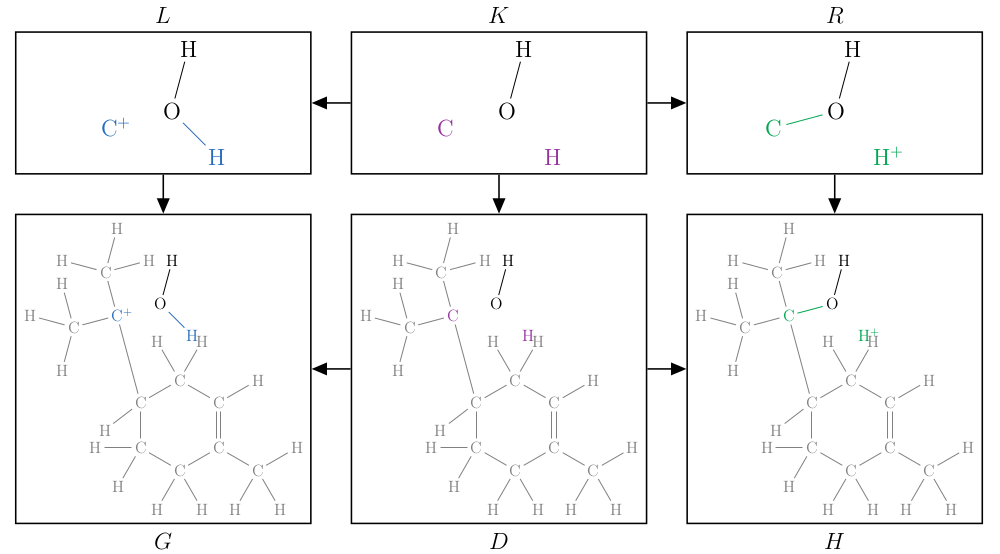
\includegraphics[width=\linewidth]{images/quenchingByWater.png}
	\caption{{Exemplo de regra por resfriamento de água e sua aplicação às moléculas $H_2O$ e $\alpha$-terpinol.}}
	\label{figRuleExample}
\end{figure}


\texttt{Med{\O}lDatschgerl}, ou  sua abreviação, \texttt{M{\O}D}, é um pacote de software inspirado quimicamente na transformação de grafo que pode direcionar um conjunto de moléculas iniciais e gerar a rede de reação química automaticamente, aplicando-se a regra baseada na transformação de grafos.  O conjunto de 17 regras de transformação de grafos, conforme as figuras abaixo, foi desenvolvido no formato GML para representar cada mecanismo de reação química encontrado na literatura. 
Essas regras transformam o conjunto inicial de moléculas ($GPP$ e $H_2O$) combinando-as em um primeira iteração, e gerando um novo conjunto de moléculas quimicamente possível. Então, em uma nova iteração, o conjunto de regras é novamente aplicada ao novo conjunto de compostos, gerando uma terceiro conjunto de compostos e assim por diante. Em cada simulação, é possível customizar ambos os conjuntos de regras a serem aplicados e o número de iterações. Para facilitar essa tarefa, construímos um interface Web, que trabalha offline e permite gerar um arquivo com o código de simulação de acordo com os parâmetros escolhidos. Um explicação gráfica para o método proposto é mostrado na figura ~\ref{figMethodSummary}.

\begin{figure}[H]
	\centering
	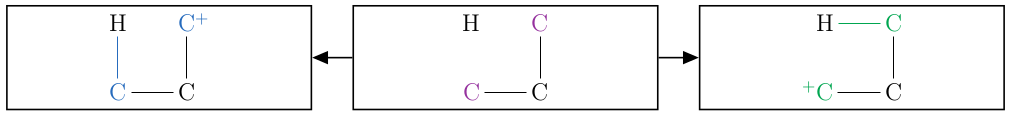
\includegraphics[width=.86\linewidth]{images/r1.png}
	\caption{\href{https://github.com/waldeyr/2PathTerpenes/blob/master/rules/1-3Hshift.gml}{1,3 hydrid shift.}}
	\label{figRule}
\end{figure}

\begin{figure}[H]
	\centering
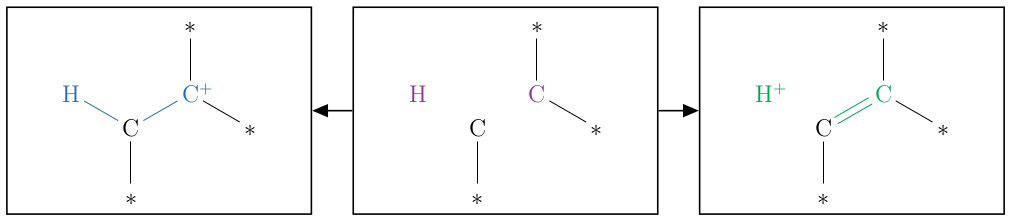
\includegraphics[width=.925\textwidth]{images/r2.png}
\caption{\href{https://github.com/waldeyr/2PathTerpenes/blob/master/rules/h_loss.gml}{Perda de $H^+$.}}
\label{figRule2}
\end{figure}

\begin{figure}[H]
	\centering
	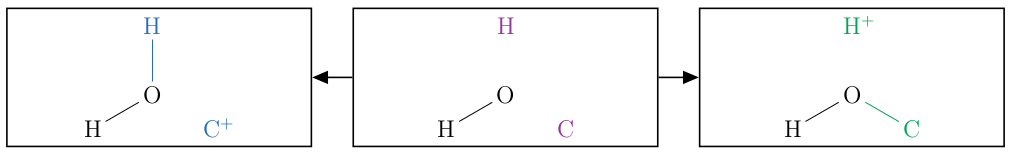
\includegraphics[width=.925\textwidth]{images/r3.png}
	\caption{\href{https://github.com/waldeyr/2PathTerpenes/blob/master/rules/h2o_gain.gml}{Captura de $H_2O$.}}
	\label{figRule3}
\end{figure}


\begin{figure}[H]
	\centering
	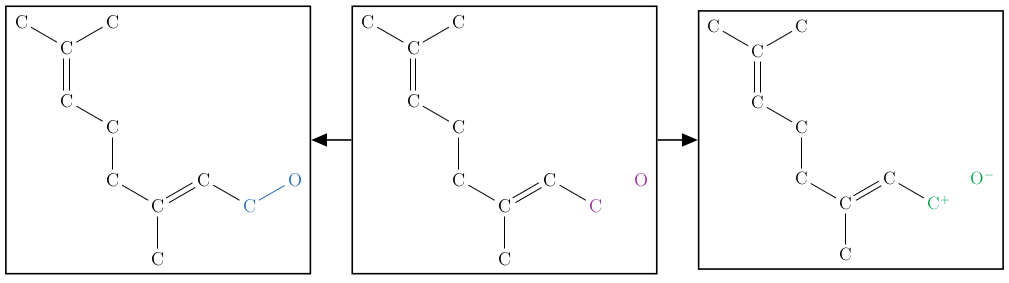
\includegraphics[width=.925\textwidth]{images/r4.png}
	\caption{\href{https://github.com/waldeyr/2PathTerpenes/blob/master/rules/opp_loss_gpp.gml}{Perda do GPP difosfato}}
	\label{figRule4}
\end{figure}

\begin{figure}[H]
	\centering
	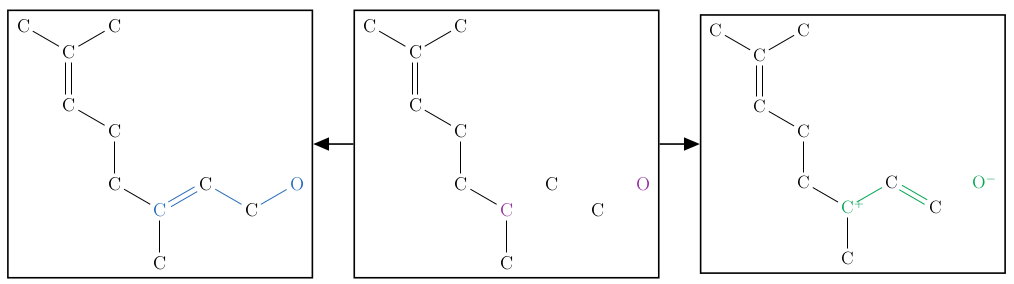
\includegraphics[width=.925\textwidth]{images/r5.png}
	\caption{\href{https://github.com/waldeyr/2PathTerpenes/blob/master/rules/opp_loss_gpp_alternative.gml}{Perda alternativa do difosfato GPP.}}
	\label{figRule5}
\end{figure}

\begin{figure}[H]
	\centering
	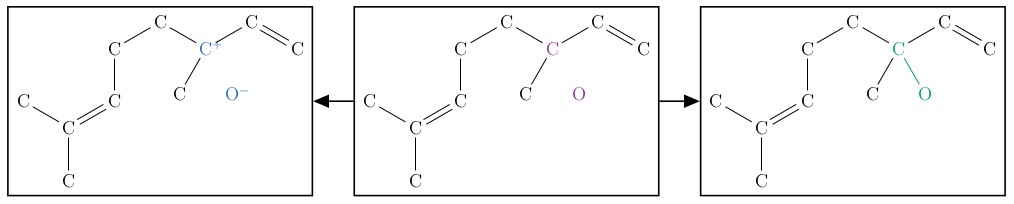
\includegraphics[width=.925\textwidth]{images/r6.png}
	\caption{\href{https://github.com/waldeyr/2PathTerpenes/blob/master/rules/opp_gain_by_geranyl_cation.gml}{Caotura de difosfato pelo geranil cátion}}
	\label{figRule6}
\end{figure}

\begin{figure}[H]
	\centering
	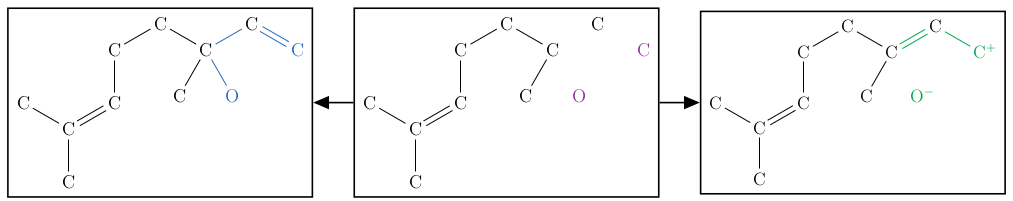
\includegraphics[width=.925\textwidth]{images/r7.png}
	\caption{\href{https://github.com/waldeyr/2PathTerpenes/blob/master/rules/opp_loss_for_lpp_c3.gml}{Perda do difosfato LPP.}}
	\label{figRule7}
\end{figure}

\begin{figure}[H]
	\centering
	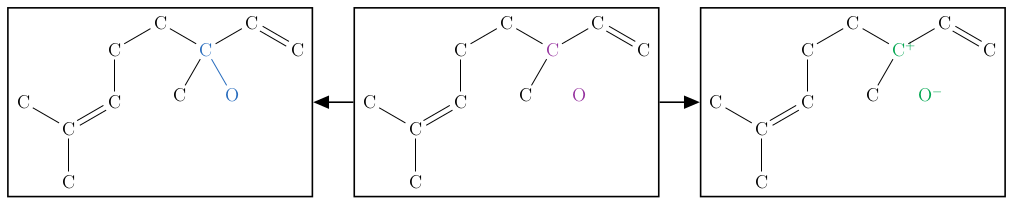
\includegraphics[width=.925\textwidth]{images/r8.png}
	\caption{\href{https://github.com/waldeyr/2PathTerpenes/blob/master/rules/opp_loss_for_lpp_c3_alternative.gml}{Perda alternativa do difosfato LPP.}}
	\label{figRule8}
\end{figure}


\begin{figure}[H]
	\centering
	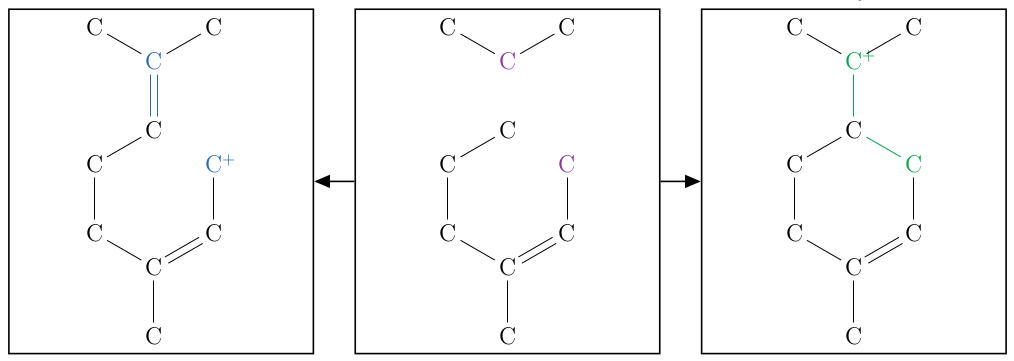
\includegraphics[width=.925\textwidth]{images/r9.png}
	\caption{\href{https://github.com/waldeyr/2PathTerpenes/blob/master/rules/1-6-closure.gml}{Fechamento do anel 1-6.}}
	\label{figRule9}
\end{figure}


\begin{figure}[H]
	\centering
	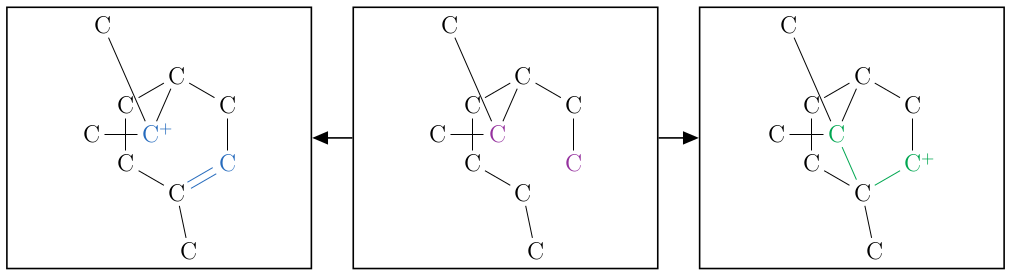
\includegraphics[width=.925\textwidth]{images/r10.png}
	\caption{\href{https://github.com/waldeyr/2PathTerpenes/blob/master/rules/3\%2C7-closure.gml}{Fechamento do anel 3-7.}}
	\label{figRule10}
\end{figure}


\begin{figure}[H]
	\centering
	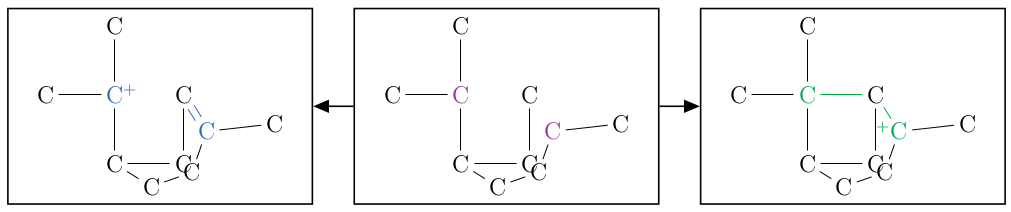
\includegraphics[width=.925\textwidth]{images/r11.png}
	\caption{\href{https://github.com/waldeyr/2PathTerpenes/blob/master/rules/2\%2C7-closure.gml}{Fechamento do anel 2-7.}}
	\label{figRule11}
\end{figure}


\begin{figure}[H]
	\centering
	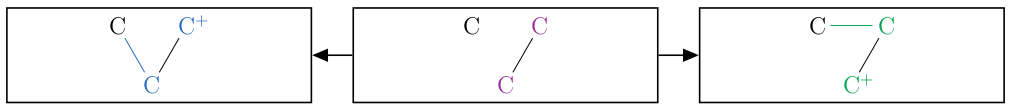
\includegraphics[width=.925\textwidth]{images/r12.png}
	\caption{\href{https://github.com/waldeyr/2PathTerpenes/blob/master/rules/WMshift.gml}{Wagner-Meerwein 1,2 alcyl shift}}
	\label{figRule12}
\end{figure}

\begin{figure}[H]
	\centering
	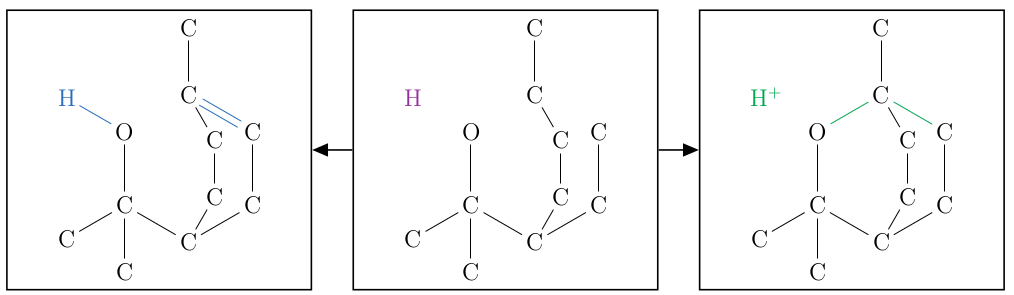
\includegraphics[width=.925\textwidth]{images/r13.png}
	\caption{\href{https://github.com/waldeyr/2PathTerpenes/blob/master/rules/1-8-cyc.gml}{Ciclização 1-8}}
	\label{figRule13}
\end{figure}


\begin{figure}[H]
	\centering
	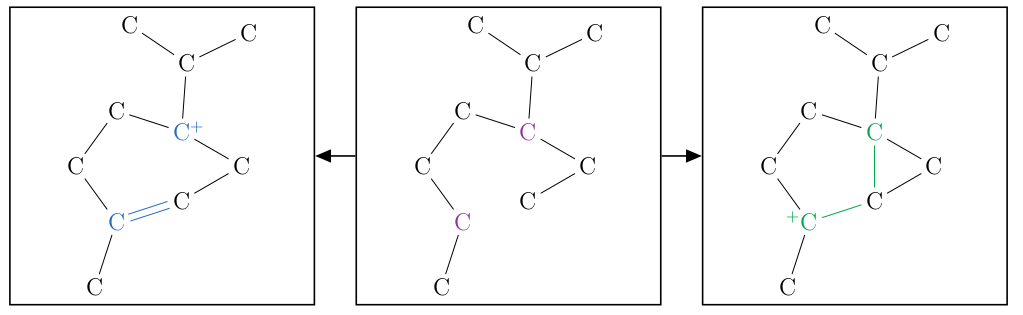
\includegraphics[width=.925\textwidth]{images/r14.png}
	\caption{\href{https://github.com/waldeyr/2PathTerpenes/blob/master/rules/2-6-closure.gml}{Fechamento 2-6}}
	\label{figRule14}
\end{figure}

\begin{figure}[H]
	\centering
	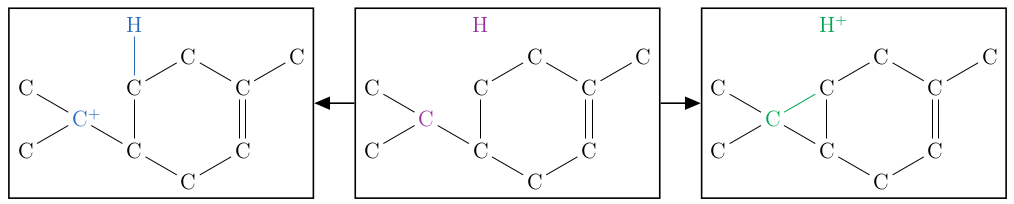
\includegraphics[width=.925\textwidth]{images/r15.png}
	\caption{\href{https://github.com/waldeyr/2PathTerpenes/blob/master/rules/5-7-closure.gml}{Fechamento 5-7}}
	\label{figRule15}
\end{figure}

\begin{figure}[H]
	\centering
	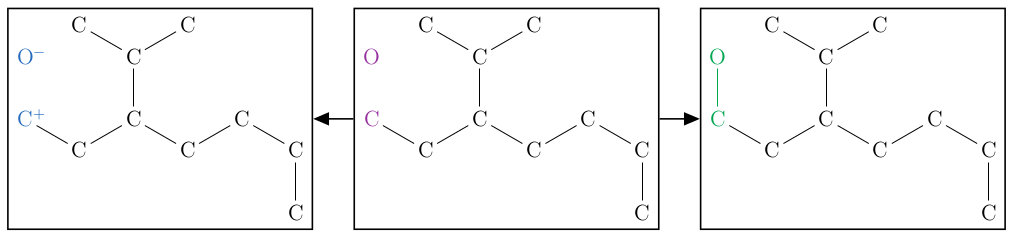
\includegraphics[width=.925\textwidth]{images/r16.png}
	\caption{\href{https://github.com/waldeyr/2PathTerpenes/blob/master/rules/opp_gain_by_bornyl_cation.gml}{Captura de difosfato pelo bornil cátion.}}
	\label{figRule16}
\end{figure}

\begin{figure}[H]
	\centering
	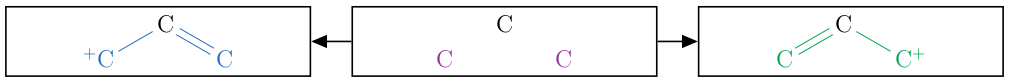
\includegraphics[width=.925\textwidth]{images/r17.png}
	\caption{\href{https://github.com/waldeyr/2PathTerpenes/blob/master/rules/allylshift.gml}{Allylic charge shift}}
	\label{figRule17}
\end{figure}


\begin{figure}[htbp]
	\centering
	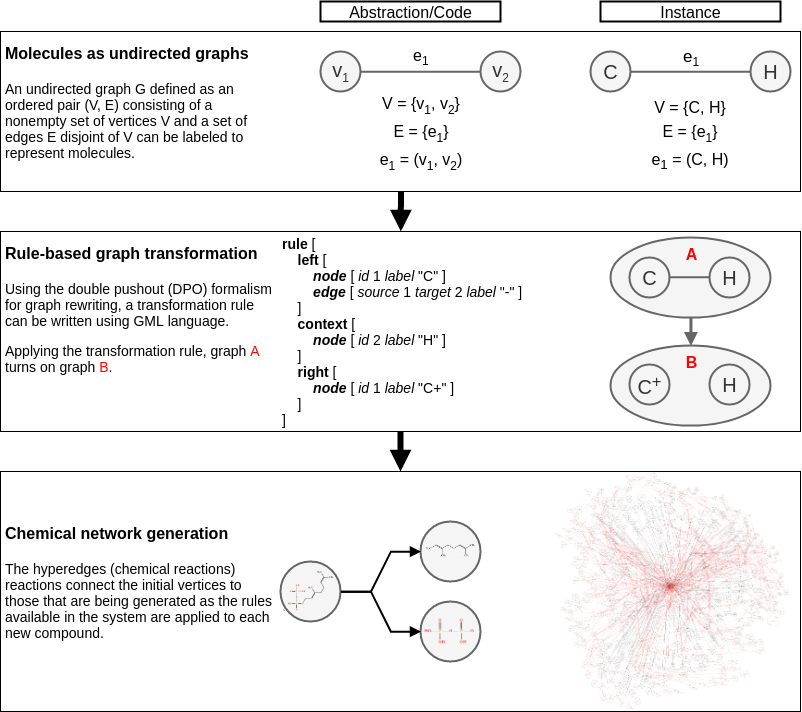
\includegraphics[width=\linewidth]{images/BIBM2019DanielaMethod.png}
	\caption{{Método resumido com exemplos de códigos/abstrações e suas aplicações para geração da rede química baseada nas transformações de grafos.}}
	\label{figMethodSummary}
\end{figure}


%\section{O que devo escrever aqui?}%

%Cada ferramenta, tecnologia, definições e todo o arcabouço teórico do trabalho deve estar em seu \nameref{Referencial_Teorico}.%
%Aqui, no \nameref{Metodo} você deve escrever como utilizou as ferramentas, tecnologias e outros recursos para resolver o problema proposto com vistas a alcançar seus objetivos.%
%Este não é lugar para definir nada novo.%


%Não caia na tentação de dizer aqui os resultados! Guarde-os para o \nameref{Resultados}. Muitas vezes é interessante começar a escrita, justamente pelo \nameref{Resultados}.%

%\fontshape{n}\selectfont%
%A tabela com a listagem de todas as atividades, pontuação e somatório encontra se na página de finalização do formulário.%

